%%% Time-stamp: <mainrep.tex 19:57, 17 Jul 2016 by P Sunthar>
%%% $Log:$
% This document describes how to use iitbreport style
%********************************************************************

%\documentclass[11pt,a4paper,openright]{report}
\documentclass[twoside]{iitbreport}

%% Default spacing: 1.5
%% Default font size: 12pt
%% Default font: txfonts (similar to times new roman)

%% Selectively comment out sections that you want to be left out but
%% maintaining the page numbers and other \ref
\includeonly{%
intro/introduction,
sc/sidechannel,
%lit/literature,
expt/experimental,
rnd/results,
%dec,
abs
%pub
%ack
}

%%% Some commonly used packages (make sure your LaTeX installation
%%% contains these packages, if not ask your senior to help installing
%%% the packages)

\usepackage{booktabs}
\usepackage{listings}

\graphicspath{{expt/}}
\graphicspath{{sc/}}


%%% Macro definitions for Commonly used symbols
\newcommand{\Rey}{\ensuremath{\mathrm{Re}}}
\newcommand{\avg}[1]{\ensuremath{\overline{#1}}}
\newcommand{\tenpow}[1]{\ensuremath{\times 10^{#1}}}
\newcommand{\pder}[2]{\ensuremath{\frac{\partial#1}{\partial#2}}}

% Referencing macros
\newcommand{\Eqref}[1]{Equation~\eqref{#1}}
\newcommand{\Tabref}[1]{Table~\ref{#1}}
\newcommand{\Figref}[1]{Fig.~\ref{#1}}
\newcommand{\Lstref}[1]{Listing~\ref{#1}}
\newcommand{\Appref}[1]{Appendix~\ref{#1}}
\newcommand{\Citeref}[1]{\cite{#1}}

\setlength{\parindent}{7pt}

\begin{document}

%%********************************Frontmatter***********************
% In frontmatter everything comes with roman numbering
\pagenumbering{roman}
\setcounter{page}{1}

%*******************************************************************
%                         Title Page
%*******************************************************************
\title{Survey of Hardware Security in Modern CPUs and GPGPUs}
\author{Meet Udeshi}

%% Print the date. Today's date comes by default, change it here to
%% other date format, if required:

%\date{\today}
%\date{10 Mar 2016}


%% The type of the report can be set here

\reporttype{Phase 1 Report}
%\reporttype{A Thesis}
%\reporttype{A Dissertation}
%\reporttype{A Project Report}

%% Name of the degree
\degree{Dual Degree Project}
%\degree{Master of Technology}


%% Department/Centre Name
\dept{Department of Electrical Engineering}

%% Supervisor and cosupervisor/excosupervisor are not essential parts
%% of a report title page, as it is your report!

%% But if you **have** to put it uncomment these
\supervisor{Prof. Virendra Singh}
%\cosupervisor{Co-super name}
%\excosupervisor{External Supervisor}

%% Roll number
\rollnum{Roll No. 14D070007}

\maketitle

%*******************************************************************
%                         Copyright Page
%*******************************************************************
%\mycopyright

%*******************************************************************
%                         Dedication Page
%*******************************************************************
%\dedication[Dedicated to \ldots]
%\addintoc{Dedication}

%*******************************************************************
%                        Certificate Page
%*******************************************************************
%\makecertificate[change title name]{report type}
%\makecertificate{seminar report}
%\makecertificate{thesis}
%\makecertificate{dissertation}
%\makecertificate{project report}

%\addintoc{Certificate}

%*******************************************************************
%                         Approval Sheet
%*******************************************************************
%\makeapproval{thesis}
%\makeapproval{dissertation}

%*******************************************************************
%                          Declaration
%*******************************************************************
%%==================================dec.tex================================
%
\begin{Declaration}
\noindent
I declare that this written submission represents my ideas in my own words and where others' ideas or words have been included, I have adequately cited and referenced the original sources. I declare that I have properly and accurately acknowledged all sources used in the production of this report. I also declare that I have adhered to all principles of academic honesty and integrity and have not misrepresented or fabricated or falsified any idea/data/fact/source in my submission. I understand that any violation of the above will be a cause for disciplinary action by the Institute and can also evoke penal action from the sources which have thus not been properly cited or from whom proper permission has not been taken when needed.

%
%
%
%
%
%
%

\DecSign[\today]



%
\end{Declaration}
%========================================================================

















%\addintoc{Declaration}

%******************************************************************
%                          Abstract
%******************************************************************
%%============================= abs.tex================================
\begin{Abstract}

    The current trends in computer architecture are increasingly 
    focusing on sharing computing resources among multiple programs
    and processes.
    Virtualisation technology and Virtual machines allow different 
    programs to share the same hardware resources.
These shared resources include all the structures inside cores and multi-core processors
which can be accessed simultaneously by threads colocated on a single core, or even processes
on two different cores. This poses a threat to the data security of many critical
processes which run in such a shared context.

Attackers with the right knowledge and tools
can leverage hardware implementation flaws in the design of these shared resources
to extract data from a victim process via undetectable side-channels. Malicious trojans
can use these shared resources to construct covert-channels to establish inter-process
communication undetectable by the core or OS. With the rapid increase of need of
powerful computation resources, GPUs have been extended to support general purpose computing.
More recently, multiple processes are able to share the GPGPU resource
and this opens up a new domain of security attacks which can be mounted on GPGPUs.

With the recent Meltdown \Citeref{meltdown} and Spectre \Citeref{spectre} attacks capable of compromising any Intel core 
regardless of the OS, it is obvious that along with power and performance, design of
computer architecture needs to consider data security as an important metric.
Moreover, a lot of software based attacks like buffer overflow and return-oriented
programming can be thwarted effectively using additional hardware structures.
Hardware support for security against software exploits is an efficient mitigation
and should also be considered when designing processors.\\
\\

In this report, an outline of recent security attack methods and mitigations
on both CPU and GPGPU is presented. The attacks range from side-channels and covert-channels over
various CPU resources to different types of return-oriented programming exploits.
Hardware-based mitigations and their effectiveness over software implementations is shown.
The literature survey is followed with an implementation of cache reverse-engineering procedure
and results.
%
%
%
%
%
\end{Abstract}
%=======================================================================



%******************************************************************
%                         Contents list
%******************************************************************
\figurespagefalse
\tablespagefalse
\makecontents % Creats toc, lof, and lot

%******************************************************************
%                        Notations
%******************************************************************
\notations[4cm]{List of Symbols}

%%********************************Mainmatter***********************
% In mainmatter everything comes with arabic numbering
\cleardoublepage
\setcounter{page}{1}
\pagenumbering{arabic}

%******************************************************************
%                         Chapters
%******************************************************************
\chapter{Introduction}

In recent years, it has become difficult to keep up with Moore's law using
conventional transistor scaling. Computer architecture has shifted
focus from optimizing single-thread performance to increasing throughput by
running multiple threads and multiple programs simultaneously.
The current trends are increasingly focusing on sharing
computing resources among multiple programs and processes.
Multi-thread and multi-core processors are commonplace in
personal computers and mobile phones, even embedded devices.
In cloud computing, technologies like virtual machines and virtual environments
are allowing multiple different programs to share the same computing resources.
These shared resources include all the structures inside cores and multi-core
processors which can be accessed simultaneously by threads colocated on a single
core, or even processes on two different cores.
This poses a threat to the data security of many critical
processes which run in such a shared context.

Attackers with the right knowledge and tools can leverage hardware
implementation flaws in the design of these shared resources
to extract data from a victim process via undetectable side-channels.
Malicious trojans can use these shared resources to construct
covert-channels to establish inter-process communication undetectable
by the core or OS. With the rapid increase of need of powerful computation
resources, GPUs have been extended to support general purpose computing.
More recently, multiple processes are able to share the GPGPU resource
and this opens up a new domain of security attacks which can be mounted on GPGPUs.

With the recent Meltdown \Citeref{meltdown} and Spectre \Citeref{spectre}
attacks capable of compromising any Intel core regardless of the OS,
it is obvious that along with power and performance, design of
computer architecture needs to consider data security as an important metric.
Moreover, a lot of software based attacks like buffer overflow and return-oriented
programming can be thwarted effectively using additional hardware structures.
Hardware support for security against software exploits is an efficient mitigation
and should also be considered when designing processors.

A lot of side-channel attacks are based on caches due to their common
accessibility between different programs. Cache accesses are abstracted away
from the program hence OS-level access-restrictions do not apply on them.
Caches also have a well-defined memory to cache-line mapping which is used
by the attacker to infer memory addresses. The time-difference between
a cache-hit versus a cache-miss is also noticeable enough to be detected
by an executing program. These characteristics make the cache vulnerable to
side-channel leakages \Citeref{disruptive}.
Cache designs which try to avoid any one of these characteristics lead to severe
performance degradation. For example, if the memory to cache-line mapping is to be
avoided, a fully-associative cache may be used instead of a direct-mapped
or set-associative cache. But a fully-associative design limits the cache-size
to a value much smaller than that desired by modern programs. In fact, the decision
of moving from fully-associative caches to set-associative caches was done
to make larger cache-sizes feasible on modern hardware, and that decision cannot
be undone only for security measures without major impact on performance.

Cache designs like Newcache \Citeref{newcache} try to achieve the same level
of performance while also preventing side-channel leakage.
There are other security methods which add enough noise
to the cache to disrupt any side-channel.
The Disruptive Prefetching \Citeref{disruptive} method utilises
the function of prefetcher to generate random memory accesses to confuse an attacker
while not interfering with program execution and performance.
Another method introduces a new context-sensitive decoder \Citeref{csd}
to mask legitimate memory access instructions with extra random accesses during
instruction decode.

Side channels work best when only the targeted region of code of the victim
is making memory accesses. While it is possible to prevent other programs and
victim's irrelevant code from interfering, hardware which generates memory
accesses like the prefetcher are difficult to stop. The thesis presents an
attack on the prefetcher which tries to completely disable it from
generating any memory accesses. This will help enhance the side channel
to facilitate better and faster key extraction.

A new potential side-channel which exploits shared Reorder Buffer (ROB) in
SMT cores is presented. ROB is one shared resource which hasn't been analysed
before for potential side-channel leakages. A scenario is shown where stalls in
one thread can affect IPC of another thread sharing the same core.
% TODO add ROP attacks

% In this report, an outline of recent security attack methods and mitigations
% on both CPU and GPGPU is presented.
% The attacks range from side-channels and covert-channels over
% various CPU resources to different types of return-oriented programming exploits.
% Hardware-based mitigations and their effectiveness over software
% implementations is shown. The literature survey is followed with an
% implementation of cache reverse-engineering procedure and results.

\chapter{Side and Covert Channel Attacks}

Shared resources of the processor can leak information about the tasks
being performed in it as shown in \Figref{fig:dls}.
This leaked information may be extracted by an attacker using
various means. The attacker will try to use some form of measurement like
cache hit/miss, time of execution, power consumption, EMI spikes to determine what part of
code is running or what data is being processed \Citeref{side-channel}. These kind of attacks have been proven
to be effective on cryptography algorithms.


\begin{figure}[h]
    \centering
    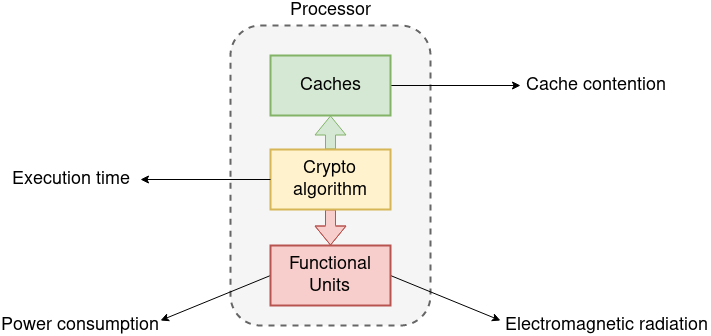
\includegraphics[width=0.7\textwidth]{side_channel.png}
    \caption[Data leakage sources]{A number of side channels which are capable of leaking data.}
    \label{fig:dls}
\end{figure}

\section{Data dependent execution in encryption algorithms}

Encryption standards like RSA, ECDSA, AES have been implemented in programs in a way
which causes certain branches and memory access patterns to be dependent on the secret key.
By using side channels to analyse which branch was taken or detect which memory address was loaded,
it is possible to decode the secret key. For example, \Lstref{lst:kdrsa} shows the key-dependent branch
of fast exponentiation part of RSA. Fast exponentiation works by repeated squaring and multiplying
when bit of the exponent is 1. In RSA, the secret key is used as the exponent hence we get
a bit-by-bit difference in executed code.
When analysing power trace or measuring timing of the execution of
this part of code, we can infer that higher power consumption and larger execution time occur
when key bit is 1. This proves that there is information being leaked bit by bit.

\begin{lstlisting}[caption={Key-dependent branch of fast exponentiation used in RSA},label={lst:kdrsa},language={C}]
while(key > 0) {
    e = key % 2;

    Square();
    Reduce();
    if(e == 1) {
        Multiply();
        Reduce();
    }

    key >>= 1;
}
\end{lstlisting}

In algorithms like AES and DES, P-box and S-box are used for fast permutation and substitution.
They essentially store a mapped permutation or substitution for each key value.
This means that during execution, AES algorithm will access various different blocks from
S-box and P-box memory region depending on the key which is being used. If we can
trace these memory accesses in some way, we can infer the secret key.
Memory buses leak data about the address via EMI channel, and by analysing that we can
get a trace of the memory access pattern.

A better and more effective way of obtaining memory access patterns is by analysing the cache.

\section{Cache side channel}

All the threads running in a single core use the same L1 caches inside that core.
Processes running on two different cores in a multi-core processor share the Last level cache.
The data access patterns of a process leaves behind fingerprints in the cache. Because of set-associativity,
if we can determine which cache line is being accessed by the process, we can determine the actual address
which was accessed.

This is done without ever having to read the actual cache line, by causing contention
on that cache line by an attacker process \Citeref{cache-side-channel}. When the attacker and victim are both trying to use the same cache
line, the attacker will get noticeable difference in execution time due to cache misses.
There are various ways in which a cache side channel can be created.

\section{Prime+Probe}

The steps followed by Prime+Probe attack are as follows:

\begin{enumerate}
\item Attacker primes the cache line by loading his own data which .
\item Victim process runs and accesses memory mapped to same cache line, hence evicting attacker's data.
\item Attacker probes the cache line by reloading the same data, and looking for a cache hit/miss.
\end{enumerate}

\begin{figure}[h]
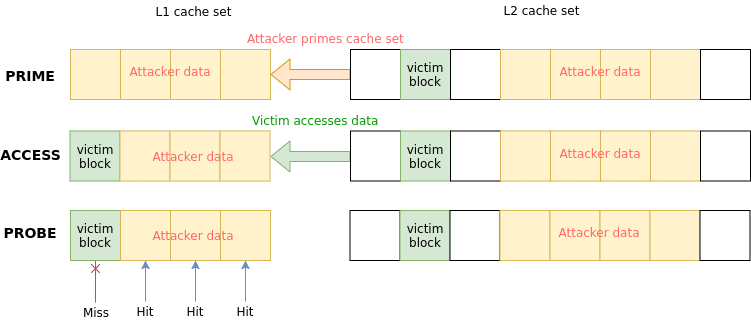
\includegraphics[width=0.9\textwidth]{prime_probe}
\caption[Prime Probe attack]{Example of a prime-probe attack on single L1 cache set. Miss in the PROBE step can be noticed by increased execution time}
\label{fig:pp}
\end{figure}

A miss in the probe step results in increased code execution time for the attacker,
which it can easily measure by reading the Time Step Counter present in many modern cores.
As shown in \Figref{fig:pp}, attacker has to prime the entire cache set (all ways) for a successful attack.
For analysing the victim's every memory access, attacker needs to prime the entire cache.
This priming step leads to a lot of cache misses and can be tracked by event counters and
trigger security exceptions when the cache misses reach an alarming amount.
Moreover, in cases where attacker and victim are not colocated on the same core,
such an attack would have to use a lower level of shared cache like LLC. The probing step
requires LLCs to be fully inclusive else the victim will not evict attacker's data from the LLC
and not lead to the required cache miss.

\section{Flush+Reload}

Flush+Reload is a side channel attack on caches which relies on the \texttt{clflush} instruction present in
X86 ISA (and similar variants in other ISAs). Flush+Reload is able to work at a finer granularity than Prime+Probe.
It is also able to successfully mount cross-core attacks via the LLC.

\begin{enumerate}
\item Attacker flushes a cache line using \texttt{clflush}.
\item Victim process runs and accesses memory hence loading the flushed block into cache.
\item Attacker reloads the same data, looking for a cache hit/miss.
\end{enumerate}

\begin{figure}[h]
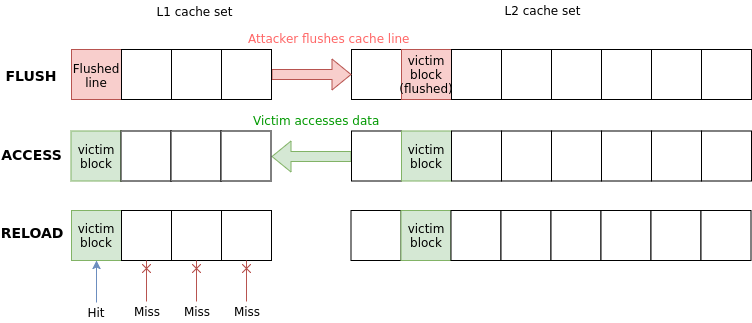
\includegraphics[width=0.9\textwidth]{flush_reload}
\caption[Flush Reload attack]{Example of a flush-reload attack on single L1 cache set. Hit in the RELOAD step can be noticed by decreased execution time}
\label{fig:fr}
\end{figure}

As seen in \Figref{fig:fr}, the granularity of Flush+Reload is at cache line level rather than cache set level.
This happens because the attacker tries to access the same data as the victim, instead of creating contention with
other data mapping to the same cache set. Accessing same data is possible because majority of encryption algorithms
are provided as system-wide shared libraries. Both the code and data regions of these libraries can be accessed by all
processes. As opposed to Prime+Probe, this makes Flush+Reload a very practical and efficient attack.
Flush+Reload is able to achieve greater granularity and accuracy due to it scanning for Cache Hit instead of Cache Miss.

\begin{figure}[h]
\centering
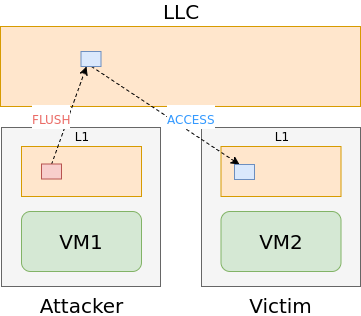
\includegraphics[width=0.5\textwidth]{flush_reload_crossvm}
\caption[Cross-VM Flush+Reload]{Flush+Reload via the LLC enables mounting Cross-VM attacks. This exploit is extremely significant in cloud computing environments}
\label{fig:crossvm}
\end{figure}

Flush+Reload is also effective on LLCs because inclusivity will not affect \texttt{clflush} behaviour, hence
attacker will get an LLC hit when the victim process accessed data. This opens up possibility of mounting a Cross-VM 
attack \Citeref{cross_vm} like shown in \Figref{fig:crossvm}

\section{Cache side channels on GPGPU}

GPGPUs have a massively parallel architecture which allows for SIMT workloads to efficiently run.
Apart from graphics and display use-cases, GPGPUs are being used for parallel computation using
frameworks like CUDA and OpenCL. GPGPUs in cloud services are specifically designed for such computational
use-cases. Nvidia GPGPUs have recently started to support concurrent kernel execution at SM level,
which allows multiple programs to simultaneously use the GPGPU resource. In this shared context,
one must look at side channels which can be exploited.

\begin{figure}[h]
\centering
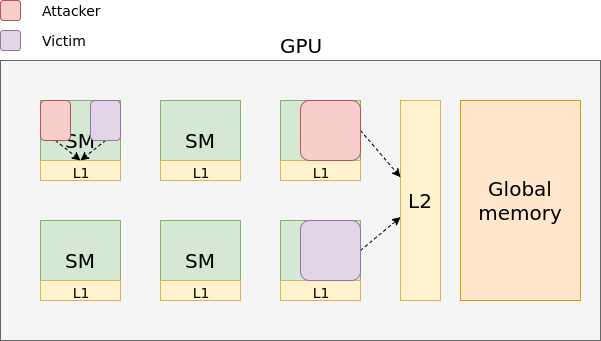
\includegraphics[width=0.7\textwidth]{gpgpu}
\caption[Memory layout of GPGPU]{GPGPU memory layout. Attacker and Victim colocation allows using L1 and L2 caches as side channels.}
\label{fig:gpgpu}
\end{figure}

The structure of GPGPU memory layout is shown in \Figref{fig:gpgpu}. Every SM contains a private L1 cache,
and all SMs share an L2 cache. The Global memory contains multiple types of memory division like Constant memory,
Texture memory etc. Concurrent kernel execution allows co-location of different kernels on same SM. Due to resource
constraints, kernels could also run on two different SMs simultaneously. The first case allows attacker to
use L1 cache as side channel, and in the second case attacker has to use L2 cache.

Mounting a side channel attack on AES is possible on GPGPU because of existing implementations of AES for GPGPU.
However, there are not many cases where encryption algorithms are run on GPGPUs. So these side channels are used
as covert channels instead. Covert channels use the same methods as side channel but they are used to set up
communication between two malicious programs. Such covert channels can be useful to leak data to third parties
without the OS or hardware detecting malicious behaviour.

% TODO naghibijou paper
\begin{figure}[h]
\centering
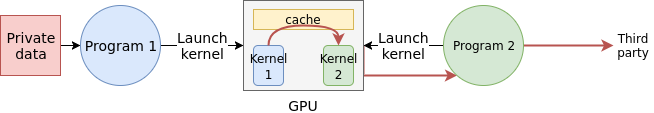
\includegraphics[width=\textwidth]{covert_channel}
\caption[Covert channel on GPGPU]{Structure of covert channel via GPGPU.}
\label{fig:gpgpu}
\end{figure}

Naghibijouybari et al in \Citeref{covert_gpgpu} achieve communication speed of over 4Mbps using
a combination of L1 cache contention and SFU contention as covert channels on multiple Nvidia GPGPU
architectures. They have used the inherent parallelism in GPGPUs to multiply the speed of the created
covert channels by opening parallel communication channels on each SM.

A critical part of their attack is reverse engineering various parameters of GPGPU architecture.
To use caches as a side channel, we need to know all parameters of the cache structure. We also need
to know of the warp scheduling policy to control colocation of two different kernels on same SM.

\section{Reverse engineering cache parameters}

This implementation of reverse engineering cache parameters is based on \Citeref{gpu_reverse}. In that paper, Wong et al
show how using a stride access pattern over an array to trigger a predictable number of cache-misses.
By measuring latency of stride access, we can get an idea of the number of cache misses.

For a given array size, we need to feed in the stride pattern into the array i.e.
\texttt{array[i]} should contain location of \texttt{array[i+STRIDE]}. We can create such an
array pattern offline before starting timing measurements. In this way, we can do a linked-list like
traversal of the array without needing to calculate next stride location online.
\Lstref{lst:offline} shows how one can create the array with a stride pattern.

\begin{lstlisting}[label={lst:offline},caption={Offline formation of array with stride access pattern},language={C}]
size_t* array; // malloced beforehand
size_t t;

for (int i=0; i<array_size; i++) {
    t = i + STRIDE:
    if(t >= array_size) t %= STRIDE;
    array[i] = (size_t)array + sizeof(size_t)*t;
}
\end{lstlisting}

For measuring timing of the array access, \texttt{rdtsc} instruction is used to get a reading of the Time Step Counter before
and after accessing the array. The difference is plot versus array size. \Lstref{lst:array_access} shows how to traverse the array
using the stride access data stored in it. The \texttt{next\_ptr} variable stores pointer to next element to access. It is dereferenced
and the loaded data is again stored into \texttt{next\_ptr} for the next iteration.

\begin{lstlisting}[label={lst:array_access},caption={Timing measurement of stride access over the entire array},language={C}]
long start = __rdtsc();
size_t* next_ptr = &array[0];
for(int i=0; i<MAX_ITERS; i++) {
    next_ptr = *((size_t**)next_ptr);
}
long time = __rdtsc() - start;
\end{lstlisting}

\Figref{fig:gem5_cache} shows a plot of latency vs array size. The latency plot stays constant initially until an array size
which fills up the whole cache. Once that happens, some lines in the cache start getting evicted and we see a steep rise in latency.
After any rise, the latency stays constant for the line size of the cache. This is obvious because any access in the same cache line
will incur same total latency as there will only be one cache miss. This latency rise occurs once for each cache set, because as
long as there are new cache sets to evict, there will be misses. The latency increase stops when one whole way of the cache is replaced
once by the array access. The starting point of latency increase gives us cache size. The step width gives us line size. Number of steps
gives number of sets, but that is hard to clearly determine when noise is present in measurements. Thus we determine way size by looking at
the point where the latency plot flattens out again. Then $\mathrm{# sets} = \frac{\mathrm{way size}}{\mathrm{line size}}$.

\subsection{Experimental setup}

For all cases, stride of 64B was used.

One set of simulations was done using gem5 simple CPU and configurable cache sizes. This was done for testing out
the algorithm. \Figref{fig:gem5_cache} was plot for L1 data cache of 1KB size, 2-way, 64B line size. \Figref{fig:gem5_cache2}
was plot for L1 data cache of 16KB size, 4-way, 64B line size.

The same algorithm was run on Intel Skylake i5-6500 processor with L1 cache of 32KB size, 8-way, 64B line size. The latency
plot is shown in \Figref{fig:x86_cache}. As is seen, there is some amount of noise due to Out-of-Order processing and
other programs interfering with the execution of the latency measurements. Despite the noise, we can clearly make out
the steps, beginning of the latency increase, and way size. This gives us every parameter required for the cache.

\begin{figure}[h]
\centering
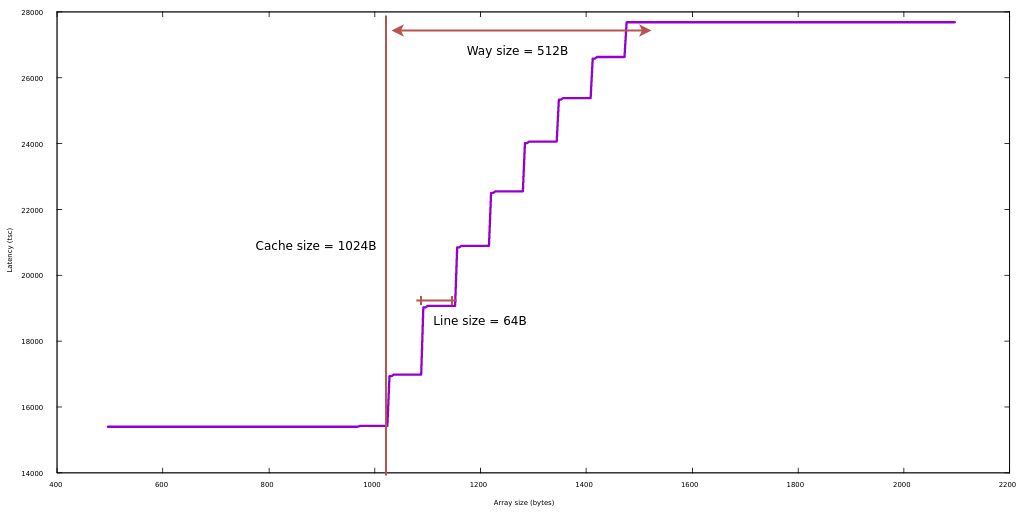
\includegraphics[width=\textwidth]{reverse_eng_1kb}
\caption[1KB cache stride access]{Latency vs. Array size plot for a 1kB 2-way cache with 64B cache line.}
\label{fig:gem5_cache}
\end{figure}

\begin{figure}[h]
\centering
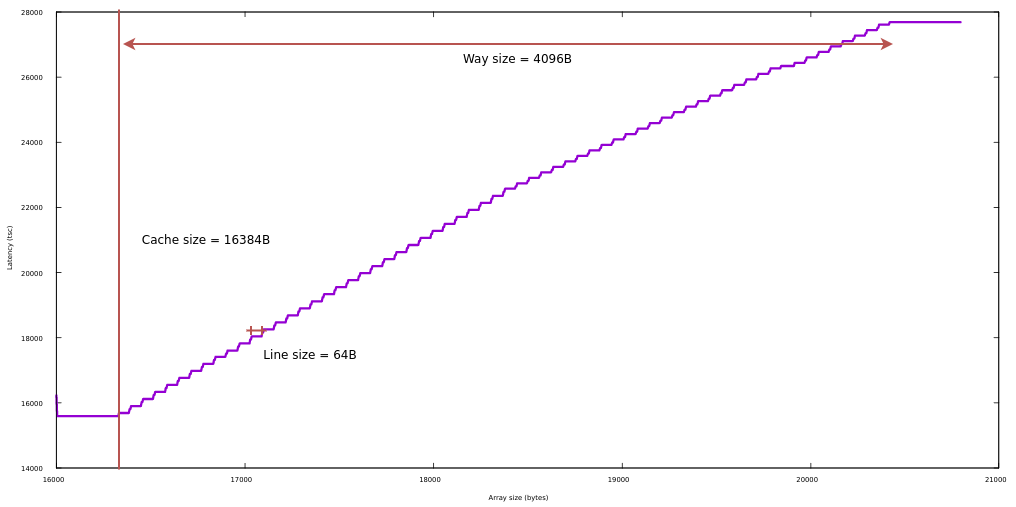
\includegraphics[width=\textwidth]{reverse_eng_16kb}
\caption[1KB cache stride access]{Latency vs. Array size plot for a 16kB 4-way cache with 64B cache line.}
\label{fig:gem5_cache2}
\end{figure}

\begin{figure}[h]
\centering
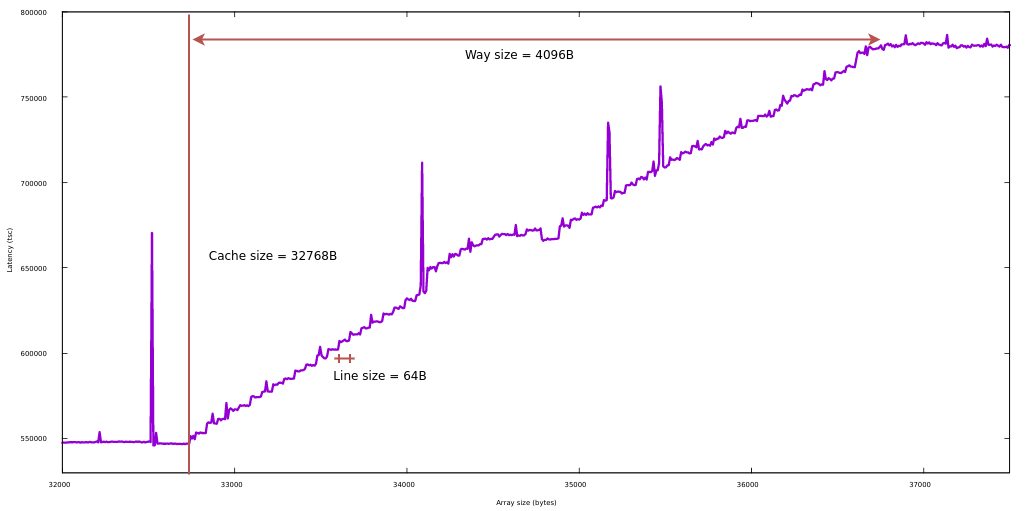
\includegraphics[width=\textwidth]{reverse_eng_32kb}
\caption[1KB cache stride access]{Latency vs. Array size plot for a 32kB 8-way cache with 64B cache line. Run on Intel Skylake i5-6500}
\label{fig:x86_cache}
\end{figure}

\chapter{Mitigations against Cache side channels}

Software based mitigations against cache side channels involve changing the
implementation of each encryption algorithm to avoid leaking data. But that is only
possible for a specific set of known attacks, and it is unavoidable for any software
to not leave some kind of fingerprint in the shared resources.

A proper solution involves changing hardware design of caches so that one process
doesn't affect other processes via its cache accesses in a predictable way.

\section{Partition-locked cache}

Cache partitioning is a naive way of isolating processes from interfering with each other's cache accesses.
A partitioned cache will let only one process access a single partition at a time \Citeref{part_cache}. If we partition
the cache statically, it is equivalent to having a private cache for every thread on the core.
This either leads to huge power and area usage or high drop in performance.

Wang et al have proposed a dynamically partitioned cache in \Citeref{pl_rp_cache}. As seen in \Figref{fig:plcache},
they add extra bits to every cache line to determine whether line is "Locked" and "ID" of thread which locked it.
A modified cache replacement policy takes into account these bits when replacing any line. This ensures that
locked lines can only be replaced by the process that locked them. Hence, other processes will not be able
to interfere with locked lines.

\begin{figure}
    \centering
    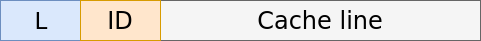
\includegraphics[width=0.7\textwidth]{pl-cache}
    \caption{A single cache line of PLCache}
    \label{fig:plcache}
\end{figure}

For implementing the PLCache, the hardware level changes include extra bits for every cache line and a change of the
replacement policy. However, PLCache requires addition of special locked-load/store instructions to the ISA. This
also means OS has to look over which process gets to use them as a fairness measure. If unchecked, attackers can intentionally
lock lines which will hinder performance of other programs. Overuse or abuse of the locking feature can lead to severe
performance degradation, if not checked by the OS.

PLCache is better than static partitioning in that it allows locked partitions of the cache to be assigned dynamically.
But it has certain drawbacks in terms of implementation.

\section{Random permutation cache}

Random-permutation cache is another cache design proposed by Wang et al in \Citeref{pl_rp_cache}.
They have added a redirection step in the address decoder of caches which uses a random permutation
table as seen in \Figref{fig:rpcache}. 
The permutation table essentially randomises the cache line in which an address will be stored.
The size of permutation table is larger than cache size (in terms of number of lines) such that there is
lesser aliasing in the permutation table. Moreover, the replacement policy is modified to update the permutation
table for every replacement, hence an attacker will not be able to decode the mapping.

\begin{figure}
    \centering
    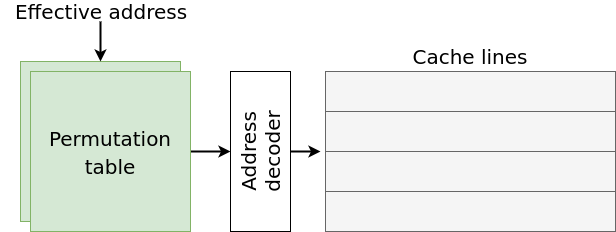
\includegraphics[width=0.7\textwidth]{rp-cache}
    \caption{Address decoding in RPCache}
    \label{fig:rpcache}
\end{figure}

RPcache is also able to mark sensitive data using "Lock" bits which are derived by page protected bit.
This is possible without any modification to ISA hence it is better than PLCache. The only drawback
of RPCache is the added step in address decoding, which will increase cache latency by one or two cycles.
This may not affect L2 or L3 caches much but it will drastically change performance of L1.
To overcome this Wang et al propose optimisations to the gate-level hardware of the decoder.
The also propose an improved cache architecture called Newcache \Citeref{newcache} which overcomes
these issues while not losing in power and performance.

\section{Intentional Cache pollution}

Cache pollution happens when unnecessary data resides in cache and evicts important data which
is being used by processes. It happens generally due to poor design and designers will
try to avoid it as much as possible, by using smarter replacement policies.

From a security perspective, we can use cache pollution to our advantage by introducing enough noise in
a cache side channel such that is hides leaked information. There are multiple ways of intentionally
polluting the cache. Two such ways are presented below.

\subsection{Disruptive Prefetching}

Pre-fetchers are hardware blocks which were originally designed to hide memory access latency
by guessing the need of certain memory address based on previous memory access patterns.
Memory locations guessed by the pre-fetcher are loaded into cache so that when the code
execution requires that memory, it gives a cache hit instead of miss. Pre-fetchers like
Stride pre-fetcher and GHB pre-fetcher are based on finding patterns in the previous memory accesses
and guessing that the next locations in that pattern will be accessed. Fuchs et al in \Citeref{disruptive}
introduce additional steps to the pre-fetchers to increase the randomness in the loaded memory address.
They randomise the pattern sequence and stride value to intentionally pollute the cache with unnecessary data.
This will degrade the performance of non-malicious programs by a bit, but will terribly disrupt any 
side channel established by an attacker. For example, in Prime+Probe attack, the attacker will not know
whether the victim or the pre-fetcher evicted its block from the cache, hence it will wrongly trace the memory
access of the victim. In the same way, Flush+Reload would get false cache hits which were not caused by the victim.

\subsection{Context sensitive decoding}

A lot of modern processors use decoders to convert from ISA to an internal instruction
representation. Most popularly Intel converts from x86 ISA to microcode using a microcode cache mapping table.
Taram et al explore in \Citeref{csd} if a custom decoder can be used to improve the security of certain programs.
They use the decoder to introduce decoy instructions in the pipeline. These decoy instructions will change the timing
characteristics of the executing program, they will pollute the cache by running decoy loads and will disrupt
attackers attempting side channel or timing attacks. Their implementation, as seen in \Figref{csd} includes adding custom decoder hardware,
and a few changes to the microcode mapping table (of which there exists an established update procedure), and a
few model specific registers to control the context of the program.
They show their method to be effective in stopping I-Cache and D-Cache side channel attacks against RSA and AES.

\begin{figure}
    \centering
    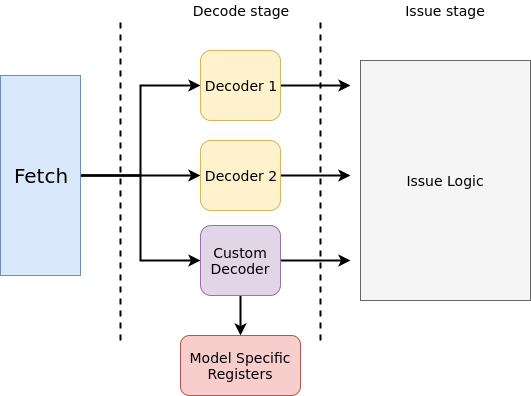
\includegraphics[width=0.7\textwidth]{csd}
    \caption{Custom decoder for context sensitive decoding}
    \label{fig:csd}
\end{figure}


%\include{lit/literature}
%\include{expt/experimental}
%\include{rnd/results}

\chapter{Conclusion}

As we saw above, the recent advances in computer architecture for performance and power gains
leads to introduction of a series of leakages from the processor which is a security concern.
It is required to design hardware by keeping security in mind as the processors get more and more
complex in order to extract higher performance gains. The industry runs a lot of security 
critical applications which if broken can cause many problems. It is important for us to
keep in mind the existance of such side channels to ensure minimal leakage of sensitive data.

%****************************************************************
%                         Appendices
%****************************************************************
%% Additional, supporting material, such as codes, derivations, etc., can be placed in the appendix
%\appendix
%\chapter{Supporting Material}

%******************************************************************
%                         Bibliography or References
%******************************************************************
%\bibliography{mylit}
\begin{thebibliography}{99}
\bibitem{side-channel}
Chenglu Jin, {\it Side Channel Attacks},
\bibitem{cache-side-channel}
D. Page, {\it Theoretical Use of Cache Memory as a Cryptanalytic Side-Channel}

\bibitem{cross_vm}
Gorka Irazoqui, Mehmet Sinan Inci, Thomas Eisenbarth, Berk Sunar,  {\it Wait a minute! A fast, Cross-VM attack on AES}
\bibitem{covert_gpgpu} 
Hoda Naghibijouybari,
Khaled N. Khasawneh,
Nael Abu-Ghazaleh, 
{\it Constructing and Characterizing Covert Channels on GPGPUs}
\bibitem{gpu_reverse}
Henry Wong, Misel-Myrto Papadopoulou, Maryam Sadooghi-Alvandi, and Andreas Moshovos, {\it Demystifying GPU Microarchitecture through Microbenchmarking}

\bibitem{part_cache}
D. Page, {\it Partitioned Cache Architecture as a Side-Channel Defence Mechanism}

\bibitem{pl_rp_cache}
Zhenghong Wang and Ruby B. Lee, {\it New Cache Designs for Thwarting Software Cache-based Side Channel Attacks}

\bibitem{newcache}
Zhenghong Wang and Ruby B. Lee, {\it A Novel Cache Architecture with Enhanced Performance and Security}

\bibitem{disruptive}
Adi Fuchs, Ruby B. Lee, {\it Disruptive Prefetching: Impact on Side-Channel Attacks and Cache Designs}

\bibitem{csd}
Mohammadkazem Taram, Ashish Venkat, Dean Tullsen, {\it Mobilizing the Micro-Ops: Exploiting Context Sensitive Decoding for Security and Energy Efficiency}

\bibitem{meltdown}
Moritz Lipp, Michael Schwarz, Daniel Gruss, Thomas Prescher, Werner Haas,
Stefan Mangard, Paul Kocher, Daniel Genkin, Yuval Yarom, Mike Hamburg, {\it Meltdown}

\bibitem{spectre}
Paul Kocher, Jann Horn, Anders Fogh, Daniel Genkin, Daniel Gruss, Werner Haas, Mike Hamburg, Moritz Lipp, Stefan Mangard, Thomas Prescher, Michael Schwarz, Yuval Yarom, {\it Spectre Attacks: Exploiting Speculative Execution}

\end{thebibliography}

%******************************************************************
%                         List of publications
%******************************************************************
%%%%
\listofpublications


\noindent Put your publications from the thesis here. The packages \texttt{multibib} or \texttt{bibtopic} or \texttt{biblatex} or enumerate environment or thebibliography environment etc. can be used to handle multiple different bibliographies in the document.








%%======================================================================
%%% Local Variables: 
%%% mode: latex
%%% TeX-master: "../mainrep"
%%% End: 









%******************************************************************
%                        Acknowledgements
%******************************************************************
%%%%
\acknowledgments

This section is for the acknowledgments. Please keep this brief and resist the temptation of writing flowery prose! Do include all those who helped you, e.g. other faculty/staff you consulted, colleagues who assisted etc.






\signature{\today}
%\signature[Indian Institute of Technology Bombay]{\today}

%========================================================================

%%% Local Variables: 
%%% mode: latex
%%% TeX-master: "../mainrep"
%%% End: 

%******************************************************************
\end{document}

%%% Local Variables:
%%% mode: latex
%%% TeX-master: t
%%% End:
